\documentclass[11pt,a4paper]{article}
\usepackage[utf8]{inputenc}
\usepackage[T1]{fontenc}
\usepackage{tgpagella}
\usepackage[spanish]{babel}
\usepackage{geometry}
\usepackage{booktabs}
\usepackage{xcolor}
\usepackage{titlesec}
\usepackage{fancyhdr}
\usepackage[parfill]{parskip}
\usepackage[expansion=false]{microtype}
\usepackage{hyperref}
\usepackage{setspace}
\usepackage{graphicx}
\usepackage{needspace}
\widowpenalty=10000
\clubpenalty=10000
\displaywidowpenalty=10000

\geometry{top=3.0cm,bottom=3.0cm,left=3.5cm,right=3.5cm}
\setlength{\parskip}{0.65em}
\setlength{\parindent}{0em}

\definecolor{azulai}{RGB}{30,80,140}
\definecolor{doradoai}{RGB}{140,90,0}
\definecolor{grisai}{RGB}{70,70,70}

\titleformat{\section}{\Large\bfseries\color{azulai}}{}{0em}{}[{\color{azulai}\titlerule[0.5pt]}]
\titlespacing*{\section}{0pt}{1.4em}{0.5em}

\titleformat{\subsection}{\large\bfseries\color{doradoai}}{}{0em}{}
\titlespacing*{\subsection}{0pt}{1.0em}{0.35em}

\titleformat{\subsubsection}{\normalsize\bfseries\color{grisai}}{}{0em}{}
\titlespacing*{\subsubsection}{0pt}{0.7em}{0.25em}

\pagestyle{fancy}\fancyhf{}
\rhead{\textcolor{grisai}{\small Izas — Arquitectura Interna}}
\lhead{\textcolor{grisai}{\small Urano · Neptuno · Plutón}}
\cfoot{\textcolor{grisai}{\small\thepage}}
\renewcommand{\headrulewidth}{0.3pt}

\hypersetup{colorlinks=true,linkcolor=azulai,urlcolor=azulai}
\setstretch{1.25}
\tolerance=1500
\emergencystretch=4em

\begin{document}

% ── Portada ──────────────────────────────────────────────────────────────────
\begin{titlepage}
  \centering
  \vspace*{1.5cm}
  {\Huge\bfseries\color{azulai} Urano · Neptuno · Plutón}\\[0.5cm]
  {\large\color{grisai} Arquitectura Interna}\\[0.3cm]
  {\small\itshape\color{grisai} Procesos profundos de cambio, sensibilidad y transformación}\[2cm]
  {\huge\color{doradoai} Izas}\\[1.5cm]
  {\Large 16/04/1979 \quad 04:20}\\[0.3cm]
  {\Large Pamplona, España}\\[0.3cm]
  {\normalsize Lat: 42.8157° \quad Lon: -1.6522° \quad UTC+02:00}\\[0.3cm]
  {\normalsize Ascendente: Acuario 6°20' \quad
    MC: Escorpio 29°12'}\\[2cm]
  \begin{tabular}{ll}
    \textbf{Urano:}   & Escorpio — Casa 9 19°58' (retrógrado)  \\
    \textbf{Neptuno:} & Sagitario — Casa 11 20°21' (retrógrado) \\
    \textbf{Plutón:}  & Libra — Casa 8 17°38' (retrógrado) \\
  \end{tabular}\\[2cm]
  \vfill
  {\small Generado el 19/05/2026}
\end{titlepage}

\tableofcontents
\newpage

% ── Datos de referencia ───────────────────────────────────────────────────────
\section{Datos de referencia}

\begin{center}
\begin{tabular}{llll}
  \toprule
  \textbf{Planeta} & \textbf{Signo} & \textbf{Casa} & \textbf{Posición} \\
  \midrule
  Urano (retrógrado)    & Escorpio   & 9   & 19°58'  \\
  Neptuno (retrógrado) & Sagitario  & 11  & 20°21' \\
  Plutón (retrógrado)  & Libra  & 8  & 17°38' \\
  Sol              & Aries  & 2  & 25°31' \\
  Luna             & Sagitario & 10 & 8°24' \\
  Ascendente       & Acuario          & ---                   & 6°20' \\
  Medio Cielo      & Escorpio           & ---                   & 29°12' \\
  \bottomrule
\end{tabular}
\end{center}

\vspace{0.5cm}
\textbf{Aspectos relevantes:}

\begin{center}
\begin{tabular}{lllll}
  \toprule
  \textbf{Planeta 1} & \textbf{Asp.} & \textbf{Planeta 2} & \textbf{Tipo} & \textbf{Orbe} \\
  \midrule
  Lilith & tri & Neptuno & Trígono & 0.3° \\
  Lilith & cua & Urano & Cuadratura & 0.7° \\
  Neptuno & cua & Venus & Cuadratura & 1.1° \\
  Urano & tri & Venus & Trígono & 1.5° \\
  Neptuno & sex & Plutón & Sextil & 2.7° \\
  Lilith & sex & Plutón & Sextil & 3.0° \\
  Neptuno & tri & Sol & Trígono & 5.2° \\
  Plutón & opo & Sol & Oposición & 7.9° \\
  \bottomrule
\end{tabular}
\end{center}

\begin{center}
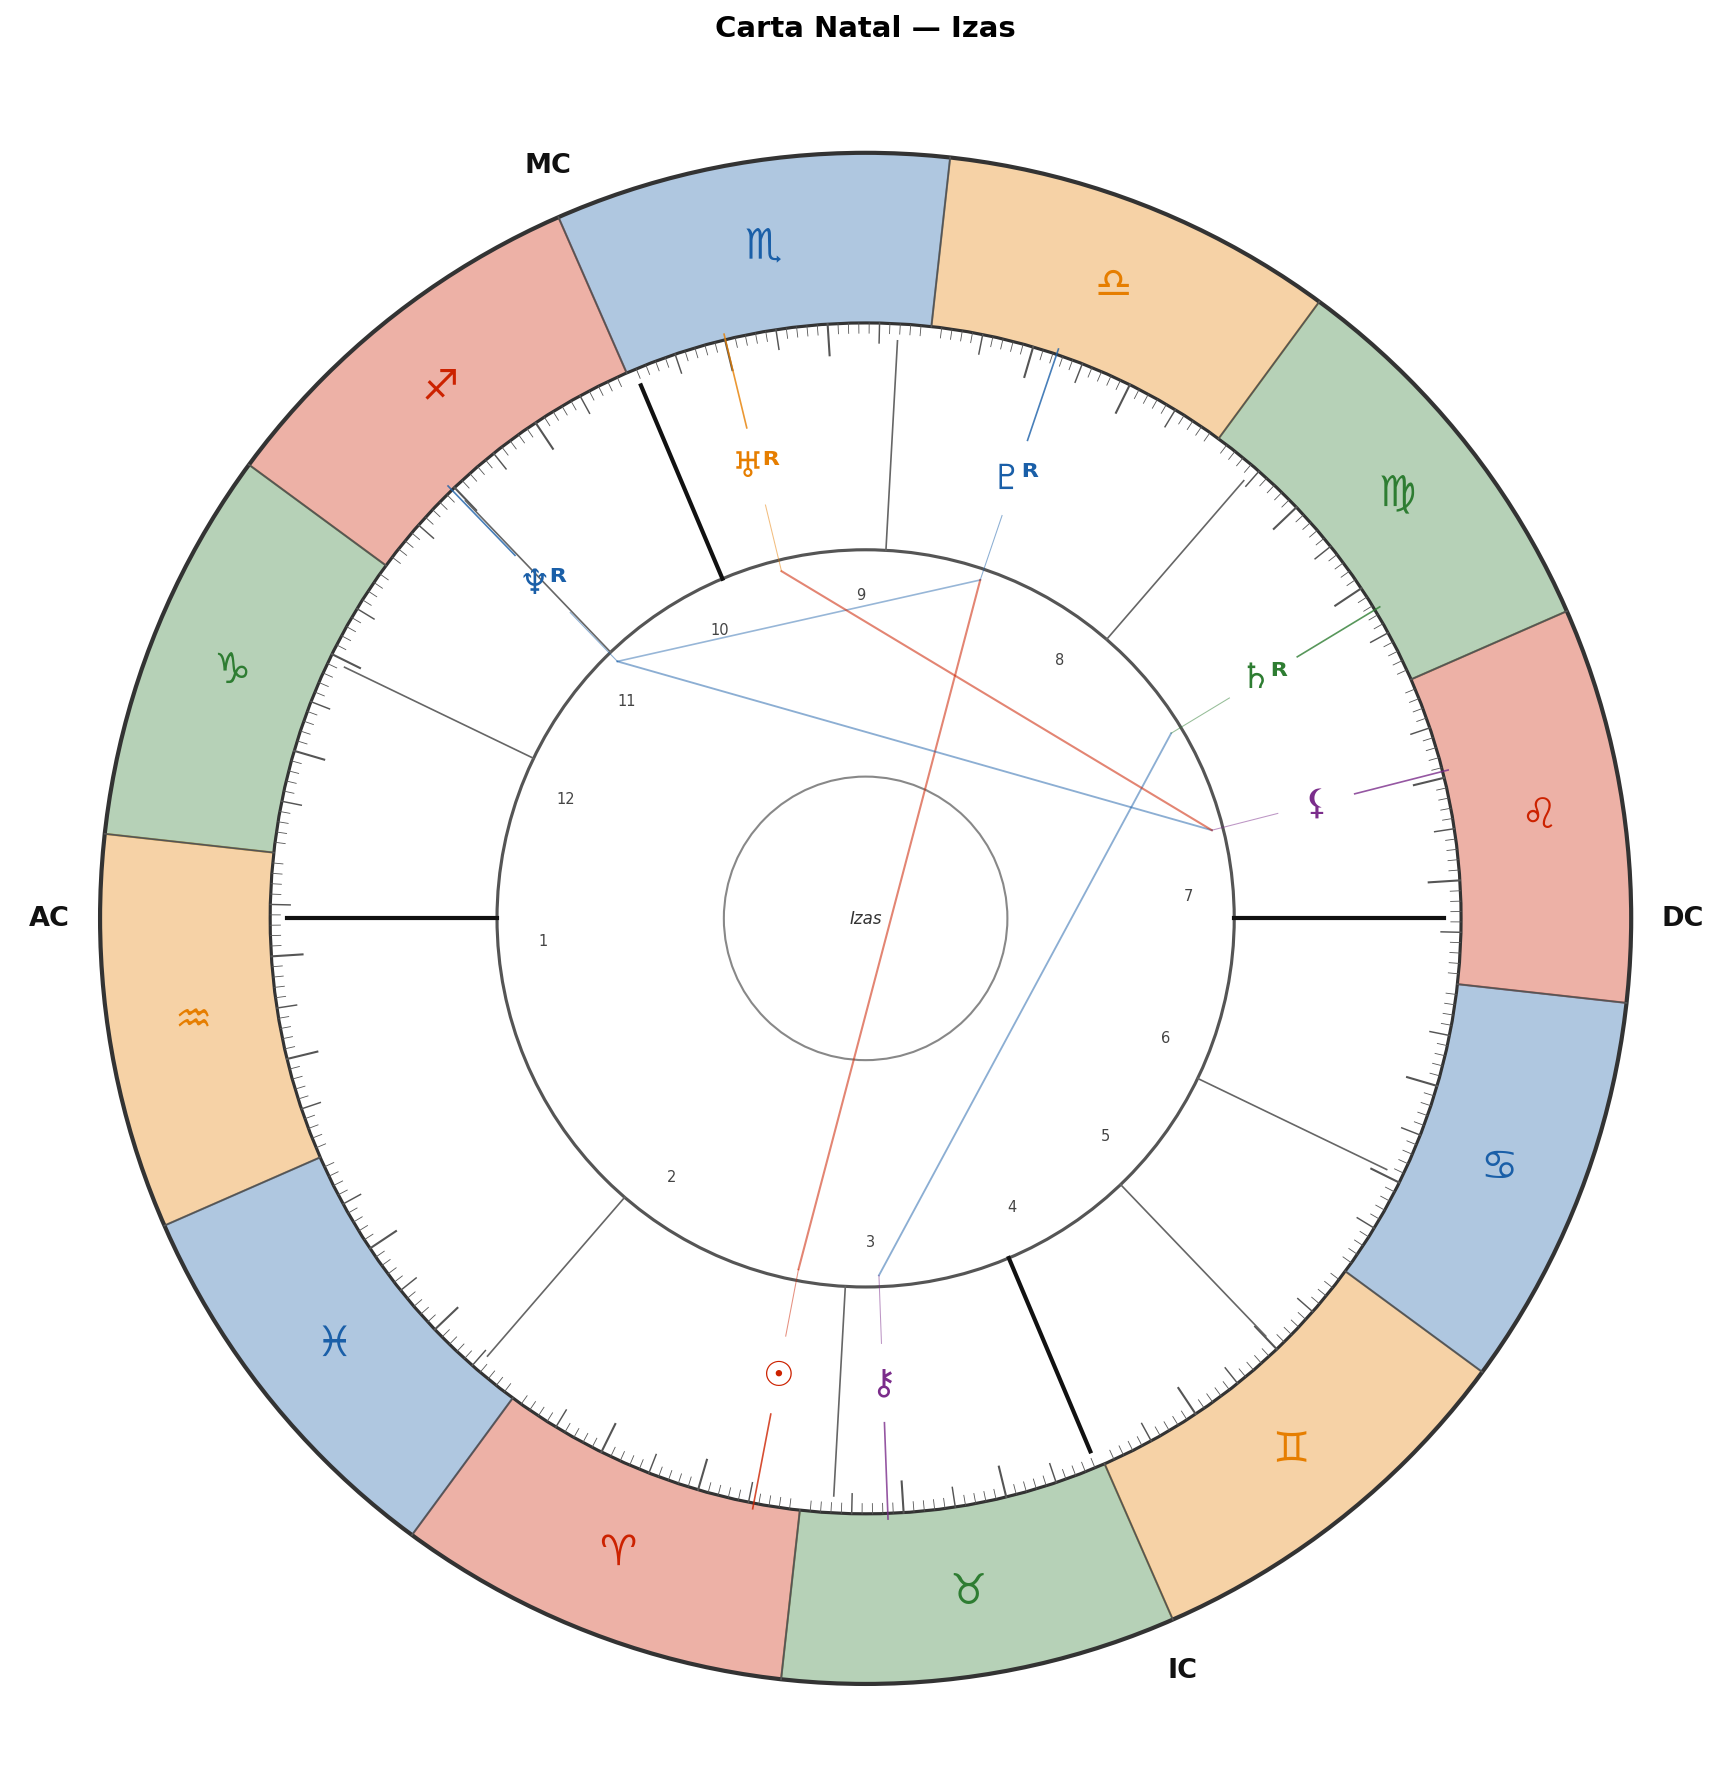
\includegraphics[width=0.72\textwidth]{Izas_rueda.png}
\end{center}

\Needspace{3\baselineskip}


% ── Interpretación ────────────────────────────────────────────────────────────
\section{Interpretación — Arquitectura Interna}

\begin{center}
{\small\itshape
No se trata de describir la personalidad. Se trata de mostrar qué procesos\\
de cambio, sensibilidad y transformación pueden activarse en tu vida.
}
\end{center}

\vspace{0.8cm}
\Needspace{5\baselineskip}

% ── 1. Marco general ──────────────────────────────────────────────────────────
\subsection{1. Marco general}

Urano, Neptuno y Plutón no describen lo más cotidiano o visible de tu carta. Muestran procesos más profundos, menos controlables, que pueden modificar tu forma de vivir, sostenerte y atravesar determinadas etapas.

Urano en Escorpio, Casa 9: muestra dónde aparecen cambios, interrupciones o necesidad de libertad. Cuando se activa, algo que antes funcionaba puede dejar de hacerlo igual.
Neptuno en Sagitario, Casa 11: muestra dónde los límites se vuelven más sensibles, difusos o permeables. Cuando se activa, algo que parecía claro puede perder forma.
Plutón en Libra, Casa 8: muestra dónde aparecen procesos intensos de transformación. Cuando se activa, algo que se sostenía de una manera ya no puede seguir igual.

Aspectos activos con planetas personales: Urano–Venus en trígono (orbe 1.53°), Neptuno–Sol en trígono (orbe 5.17°), Neptuno–Venus en cuadratura (orbe 1.15°), Plutón–Sol en oposición (orbe 7.88°).

\vspace{0.8cm}
\Needspace{5\baselineskip}


% ── 2. Urano ──────────────────────────────────────────────────────────────────
\subsection{2. Urano — Ruptura y cambio de patrón}

\subsubsection*{Urano en Escorpio — Casa 9 (retrógrado)}

Urano en Escorpio muestra cambios intensos y difíciles de controlar en procesos emocionales profundos. Hay una necesidad constante de transformación, incluso cuando una parte de ti preferiría mantener el control.

Puede haber rupturas internas importantes, descubrimientos difíciles de ignorar o momentos donde algo cambia de forma irreversible. A veces lo que intentabas contener termina emergiendo de golpe.

El aprendizaje está en permitir transformación sin vivir cada cambio como una amenaza que necesitas controlar completamente.

Urano en Casa 9 muestra necesidad de revisar ideas, creencias y formas de entender la vida. Puede costarte sostener durante mucho tiempo visiones demasiado cerradas o rígidas.

A veces cambias de perspectiva de forma bastante rápida porque necesitas volver a sentir amplitud y apertura. También puede haber giros importantes en estudios, filosofía de vida o dirección vital.

El aprendizaje está en abrir nuevas perspectivas sin perder completamente el hilo de tu propio camino.

Urano está retrógrado. Los cambios tienden a sentirse primero por dentro. Puede pasar tiempo antes de que se vean fuera, pero internamente algo ya está moviéndose, reorganizándose o dejando de funcionar como antes.

Urano en trígono a Venus facilita vivir los vínculos desde mayor libertad y autenticidad. Los cambios afectivos suelen integrarse con más naturalidad.

Puede haber apertura a relaciones poco convencionales o facilidad para adaptarte a nuevas formas de compartir.

El aprendizaje pasa por sostener los vínculos también en el tiempo, no solo en la intensidad del cambio.

\vspace{0.8cm}
\Needspace{5\baselineskip}

% ── 3. Neptuno ────────────────────────────────────────────────────────────────
\subsection{3. Neptuno — Disolución y pérdida de forma}

\subsubsection*{Neptuno en Sagitario — Casa 11 (retrógrado)}

Neptuno en Sagitario puede hacer que busques sentido, dirección o verdad en lugares que después resultan menos sólidos de lo que parecían. A veces necesitas creer en algo para sentir orientación, incluso cuando todavía no está claro.

Puede haber idealización de caminos, proyectos, filosofías o personas que parecen ofrecer amplitud o propósito. También puedes cambiar varias veces de dirección buscando una referencia más auténtica.

El aprendizaje está en desarrollar una visión más consciente sin perder apertura ni capacidad de inspiración.

Neptuno en Casa 11 puede hacer que idealices grupos, amistades o proyectos colectivos. A veces buscas pertenecer a espacios que parecen muy inspiradores pero después muestran menos claridad o coherencia real.

Puede costarte distinguir qué vínculos colectivos son realmente sostenibles y cuáles funcionan más desde expectativa o proyección.

El aprendizaje pasa por participar en lo colectivo sin perder discernimiento ni referencia propia.

Neptuno está retrógrado. La sensibilidad, la confusión o la pérdida de claridad tienden a vivirse primero internamente. Puede costarte detectar desde fuera cuándo algo está perdiendo forma, porque el proceso empieza en capas más silenciosas.

Neptuno en trígono al Sol facilita integrar sensibilidad, intuición y dirección personal. La imaginación y la inspiración suelen alimentar tu camino de forma bastante natural.

Puede haber capacidad para conectar con experiencias profundas sin perder completamente la referencia de quién eres o hacia dónde vas.

El aprendizaje pasa por dar forma concreta a lo que imaginas o percibes internamente.

Neptuno en cuadratura a Venus genera tensión entre necesidad de vínculo y dificultad para mantener claridad emocional y afectiva. Una parte de ti busca conexión ideal y otra necesita reconocer la realidad de lo que está viviendo.

Puede haber idealización de relaciones, dificultad para poner límites o tendencia a sostener vínculos poco claros durante demasiado tiempo.

El aprendizaje pasa por construir relaciones más conscientes sin cerrar la sensibilidad afectiva.

\vspace{0.8cm}
\Needspace{5\baselineskip}

% ── 4. Plutón ─────────────────────────────────────────────────────────────────
\subsection{4. Plutón — Intensidad y transformación profunda}

\subsubsection*{Plutón en Libra — Casa 8 (retrógrado)}

Plutón en Libra intensifica profundamente los vínculos y la necesidad de equilibrio real en las relaciones. Las transformaciones suelen aparecer a través de acuerdos, rupturas o dinámicas relacionales difíciles de sostener superficialmente.

Puede haber miedo a perder vínculos importantes, relaciones muy intensas o dificultad para mantener relaciones donde no existe reciprocidad verdadera.

El aprendizaje pasa por construir vínculos más honestos y profundos sin quedar atrapade en dinámicas de dependencia o control.

Plutón en Casa 8 intensifica muchísimo los procesos emocionales profundos, las transformaciones internas y todo lo relacionado con pérdida, cambio y regeneración. Las experiencias suelen vivirse con gran intensidad emocional.

Puede haber necesidad de comprender lo oculto, atravesar procesos internos muy profundos o sensación de que determinadas etapas cambian completamente tu forma de vivir.

El aprendizaje pasa por permitir transformación profunda sin vivir constantemente desde el control o la amenaza.

Plutón está retrógrado. La intensidad y la transformación tienden a dirigirse primero hacia dentro. Puede haber procesos profundos que no se ven claramente desde fuera hasta que ya han acumulado mucha fuerza.

Plutón en oposición al Sol intensifica la tensión entre identidad personal y procesos profundos de cambio. A veces sientes que cuanto más intentas sostener una dirección fija, más fuerza aparece empujando hacia la transformación.

Puede haber relaciones intensas con poder, control o experiencias que cambian profundamente tu manera de vivir.

El aprendizaje está en encontrar una forma de sostenerte sin necesitar controlar completamente cada proceso.

\vspace{0.8cm}
\Needspace{5\baselineskip}

% ── 5. Integración ────────────────────────────────────────────────────────────
\subsection{5. Integración — Las tres fuerzas en tu carta}

Urano, Neptuno y Plutón actúan de formas distintas y no siempre coordinadas. Urano en Escorpio, Casa 9, muestra dónde aparecen cambios, interrupciones o necesidad de libertad. Cuando se activa, algo que antes funcionaba puede dejar de hacerlo igual. Neptuno en Sagitario, Casa 11, muestra dónde los límites se vuelven más sensibles, difusos o difíciles de sostener. Cuando se activa, algo que parecía claro puede perder forma. Plutón en Libra, Casa 8, muestra dónde aparecen procesos intensos de transformación. Cuando se activa, algo que sostenías de una manera ya no puede seguir igual.

Neptuno en Sagitario muestra una sensibilidad especial en ciertas áreas de tu vida: tiendes a desbordarte por exceso de impulso o dificultad para frenar a tiempo. Urano en Escorpio muestra cómo suelen producirse los cambios importantes: los cambios aparecen cuando cambia lo que sientes profundamente. Plutón en Libra concentra la intensidad en procesos que no pueden quedarse igual indefinidamente: determinadas experiencias terminan empujándote a transformar algo en profundidad.

En determinados momentos, estas tres fuerzas pueden activarse de forma encadenada. Urano en Escorpio suele aparecer primero: cambian vínculos, emociones o sensaciones de pertenencia de forma repentina. Después, Neptuno en Sagitario puede hacer que aparezca sensación de confusión, pérdida de claridad o dificultad para entender bien qué está pasando: la energía pierde dirección y cuesta saber hacia dónde moverte. Finalmente, Plutón en Libra concentra la intensidad en aquello que ya no puede seguir igual: la intensidad se concentra en pensamientos, conversaciones o formas de comprender la vida. Por eso, determinadas etapas pueden sentirse especialmente intensas: no estás viviendo una sola cosa, sino varios procesos moviéndose al mismo tiempo.

\vspace{0.8cm}
\Needspace{5\baselineskip}

% ── 6. Orientación ────────────────────────────────────────────────────────────
\subsection{6. Orientación}

\subsubsection*{Cuando Urano está activo}
Urano suele activarse cuando: aparecen cambios emocionales o relacionales difíciles de prever. Esto suele sentirse especialmente en temas relacionados con la Casa 9.

\subsubsection*{Cuando Neptuno está activo}
Neptuno suele activarse cuando: pierdes claridad sobre hacia dónde quieres dirigirte. Esto suele sentirse especialmente en temas relacionados con la Casa 11.

\subsubsection*{Cuando Plutón está activo}
Plutón suele activarse cuando: determinados pensamientos o conversaciones adquieren mucha intensidad y profundidad. Esto suele sentirse especialmente en temas relacionados con la Casa 8.

\subsubsection*{Cuando no se reconocen}
Cuando estos procesos no se reconocen, es fácil vivirlos únicamente como problemas externos o mala suerte. Sin embargo, muchas veces están mostrando que algo necesita cambiar, redefinirse o transformarse más profundamente.

Intentar sostener exactamente igual algo que internamente ya está cambiando suele generar más desgaste, más confusión o más sensación de bloqueo.

\vspace{0.6cm}
Si estos procesos se ignoran durante mucho tiempo, suelen intensificarse. Urano puede traer cambios cada vez más bruscos. Neptuno puede aumentar la sensación de confusión, desgaste o pérdida de claridad. Plutón puede concentrar tanta intensidad que determinadas situaciones ya no puedan seguir sosteniéndose igual.

Por eso, reconocer antes lo que está cambiando suele ayudar a atravesar estas etapas con más consciencia y menos ruptura.

\vspace{1cm}
\begin{center}
{\small\itshape\color{grisai}
La astrología se usa aquí como lenguaje simbólico de observación, no como definición de la persona.\
Este documento es una aproximación funcional, no un diagnóstico.
}
\end{center}

\end{document}
